%----------------------------------------------------------------------------------------
%	Inställningar och dokumentkonfiguration
%----------------------------------------------------------------------------------------

\documentclass[paper=a4, fontsize=11pt]{report} % A4-sida och 11 punkters fontstorlek

\usepackage[T1]{fontenc} % 8-bitarskodning som har 256 glyfer
\usepackage[english]{babel} % Svenskt språk
\usepackage[utf8]{inputenc} % För svenska tecken
\usepackage{dtklogos} % Logos
\usepackage{wallpaper} % Bakgrundsbild
\usepackage{fancyhdr} % Specialsidhuvud och sidfot
\usepackage{enumerate} 
\usepackage{xifthen}% provides \isempty test
\usepackage{listings}% Code examples
\usepackage{xcolor}
\newcounter{tmpc}
\lstdefinestyle{BashInputStyle}{
  language=bash,
  basicstyle=\footnotesize\ttfamily,
  numbers=left,
  numberstyle=\tiny,
  numbersep=3pt,
  frame=tb,
  columns=fullflexible,
  backgroundcolor=\color{yellow!20},
  linewidth=0.9\linewidth,
  xleftmargin=0.1\linewidth
}
% Exampels
% Inline
% \lstinline[style=BashInputStyle]´# apt-get --purge remove rubygems´.
% Multiline
% \begin{lstlisting}[style=BashInputStyle]
%    # apt-get --purge remove rubygems
% \end{lstlisting}

\pagestyle{fancyplain} % Använd sidhuvud och sidfot på alla sidor
\fancyhead[L]{Seminar 4 -- 1DV020 -- 2015 -- Server Administration} % Titel till vänster i sidhuvud
\fancyhead[C]{} % Tomt i mitten
\fancyhead[R]{} % Tomt till höger
\fancyfoot[L]{} % Tomt till vänster
\fancyfoot[C]{} % Tomt i mitten
\fancyfoot[R]{\thepage} % Sidnumrering till höger i sidfoten
\renewcommand\thesection{\arabic{section}} % Section beter sig som i dokumentklassen article

\newcommand{\win}[1]{Microsoft Windows Server\ifthenelse{\isempty{#1}}{}{ #1}}
\newcommand{\gui}[0]{``Server with a GUI''}
\newcommand{\core}[0]{Windows Server Core}
%----------------------------------------------------------------------------------------
%	TITLE SECTION
%----------------------------------------------------------------------------------------
\newcommand\BackgroundPic{
    \put(-50,-50){
    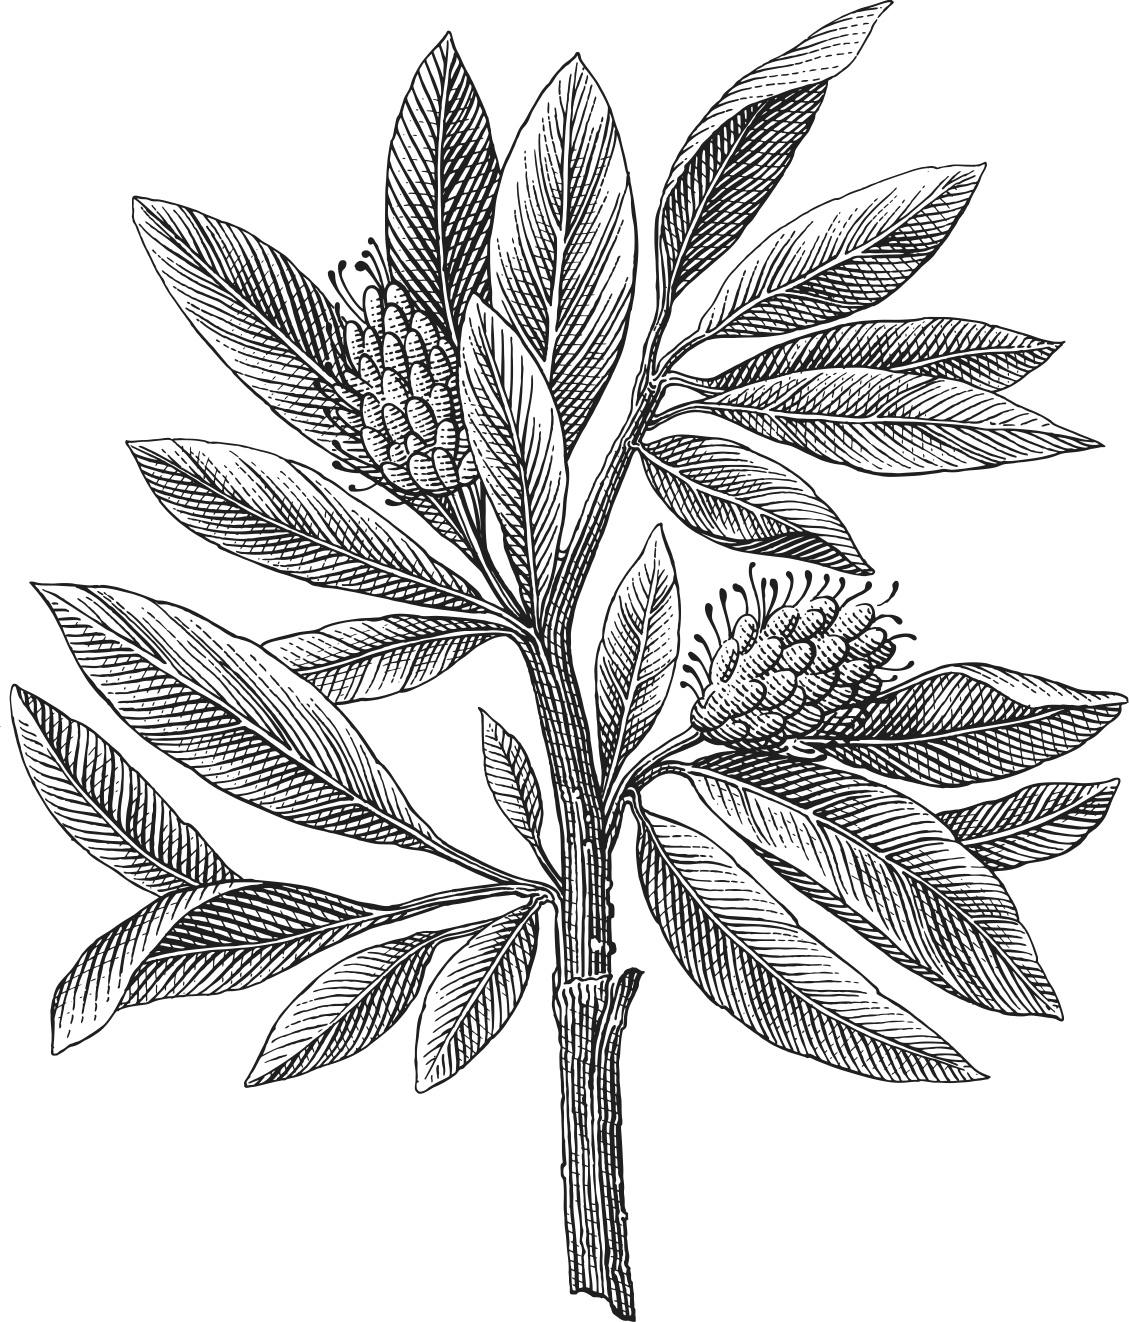
\includegraphics[keepaspectratio,scale=0.65]{lnu_etch.png} % Bakgrundsbild
    }
}
\newcommand\BackgroundPicLogo{
    \put(15,700){
    
\includegraphics[keepaspectratio,scale=0.10]{logo.png} % Logga i vänstra hörnet
    }
}

\newcommand{\horrule}[1]{\rule{\linewidth}{#1}} % Skapa hortisontell linje

\title{	\vspace{-10cm}
    \normalfont \normalsize
    \textsc{Linnaeus University} \\ [25pt] % Universitetes namn
    \horrule{0.5pt} \\[0.4cm] % Tunn linje högst upp
    \huge Seminar 4\\ % Arbetes titel
	\large \textcolor{gray}{1DV020 -- Server Administration}
    \horrule{0.5pt} \\[0.4cm] % Tunn linje längst ner
}

\author{Jacob Lindehoff} % Författarnas namn

\date{\normalsize\today} % Dagens datum

\begin{document}
\AddToShipoutPicture*{\BackgroundPic} % Lägger in backgrundsbild på första sidan
\AddToShipoutPicture*{\BackgroundPicLogo}
\maketitle % Skriv ut titeln
\noindent % Tabba inte in på första meningen

%------------------------------------------------
%	Introduktion
%------------------------------------------------
\section{Introduction}
  During this seminar, we will address the following topics:
\begin{itemize}
	\item Directory Services
	\item Active Directory
	\begin{itemize}
    	\item Overview
		\item DNS
		\item Global Catalog
		\item Organizational Units
		\item User accounts
		\item Groups
		\item User Profile
		\item Delegation of Administration
	\end{itemize}
    \item A G/U DL P
    \item Group Policy
\end{itemize}

%------------------------------------------------
%	Deadline
%------------------------------------------------
\section{Deadline}
  The seminar is on the {\color{red}4th of March 2015} and it is compulsory. If you cannot participate, it must be notified in advance and a written report of the seminar must be submitted no later than {\color{red}3 days} after the seminar. The written report should contain detailed answers to all questions in the seminar.
  \newpage
%------------------------------------------------
%	Seminariefrågor
%------------------------------------------------
\section{Seminariefrågor}

\begin{enumerate}
\begin{large}
\item Vad är en katalogtjänst och vilka användnings-områden har den?
\item Beskriv de olika delarna av Active Directory databasen.
\item Vad är Active Directory Schema och hur många scheman kan det finnas i en AD Skog?
\item Vilka delar består den logiska och den fysiska strukturen av och vad använder man dessa till?
\item Vad är en domänkontrollant?
\item Vad innehåller Globala katalogen?
\item Varför är en fungerande DNS-server så viktig för Active Directory?
\item För att skapa redundans i sin AD-miljö så installerar man en extra domänkontrollant. Det räcker dock inte med det, vad behöver man göra mer att användarna ska kunna logga in om den första domänkontrollanten går ner?’
\item Vad används Organisationsenheter till och vad är viktigt att tänka på när man skapar sin OU-struktur?
\item Vad är implicita grupper och hur skapar man en sådan?
\item Active Directory stödjer tre grupptyper, vilka är dessa?
\begin{enumerate}[a.]
	\item Var ifrån kan medlemmarna till dessa olika grupper komma?
	\item Var i skogen man använda de olika grupperna för att ge behörighet?
\end{enumerate}
\item Vad är LDAP?
\item Vilka är anledningarna till man vill köra med flera olika domänen i en skog, räcker det inte med en domän?
\item Vad skiljer en Active Directory domän från en DNS domän?
\item På vilka två sätt kan man köra inloggningsscript i en AD-miljö och beskriv hur man konfigurerar dessa?
\item Vad innehåller en Användarprofil?
\item Hur fungerar ”Roaming profile”?
\item Hur skapar man en ”Tvingande”-profil?
\item Det finns 5 stycken FSMO-roller, vilka är dessa och vad ansvarar de för?
\begin{enumerate}[a.]
	\item Hur många roller får du, om du har en skog med 5 domäner?
	\item Hur hittar du vilken DC det är som har de olika FSMO-rollerna?
	\item Hur gör du för att flytta de olika FSMO-rollerna?
\end{enumerate}
\item Read Only Domain Controller
\begin{enumerate}[a.]
	\item Vad är RODC?
	\item När ska man använda sig av detta?
	\item Hur installerar man en RODC?
\end{enumerate}
\item Med hjälp av OUn kan man delegera administration.
\begin{enumerate}[a.]
	\item Vilka olika rättigheter kan man sätta på ett OU?
	\item Hur kan detta förenkla för en IT-avdelningen?
\end{enumerate}
\end{large}
\end{enumerate}
\end{document}
